\documentclass[
    handout,
    aspectratio=169,
    12pt
]{beamer}

\usepackage{beamerstyle}
\usepackage{pgfpages}

% \setbeameroption{show notes on second screen=bottom}

\usepackage[spanish]{babel}
%

% =========================
% THEOREMS
% =========================
% \newtheoremstyle{theoremstyle}
%     {0.5em} % Space above
%     {0.5em} % Space below
%     {\itshape} % Body font
%     {} % Indent amount
%     {\bfseries} % Theorem head font
%     {.} % Punctuation after theorem head
%     { } % Space after theorem head
%     {} % Theorem head spec
% \theoremstyle{theoremstyle}
% \newtheorem{teo}{Teorema}[section]
% \newtheorem{lem}[teo]{Lema}
% \newtheorem{prop}[teo]{Proposición}
% \newtheorem{cor}[teo]{Corolario}

% \theoremstyle{definition}
% \newtheorem{defn}[teo]{Definición}
% \newtheorem{ejem}[teo]{Ejemplo}

% =========================
% THEME
% =========================
\usetheme[
    titleformat=regular,
    titlepage=moloch,
    sectionpage=none,
    titleseparator linewidth=1pt,
    numbering=fraction,
    progressbar=frametitle,
    frametitle margin top=0.2cm,
    frametitle margin left=0.5cm,
    % colortheme=catppuccin,
    colortheme=tomorrow,
    block=fill,
]{moloch}

% =========================
% TYPOGRAPHY
% =========================
% \usepackage[sfdefault]{FiraSans}
% \usepackage[T1]{fontenc}

% =========================
% COLORS
% =========================
% \definecolor{textgray}{HTML}{222222}
% \definecolor{softblue}{HTML}{4C6378}
% \definecolor{lightgray}{HTML}{E9ECEF}

% \setbeamercolor{normal text}{
%     fg=textgray,
%     bg=white
% }

% \setbeamercolor{frametitle}{
%     fg=textgray,
%     bg=white
% }

% \setbeamercolor{title}{
%     fg=textgray
% }

% \setbeamercolor{subtitle}{
%     fg=softblue
% }

% \setbeamercolor{progress bar}{
%     fg=softblue,
%     bg=lightgray
% }

% \setbeamercolor{alerted text}{
%     fg=softblue
% }

% \setbeamercolor{itemize item}{
%     fg=softblue
% }

% =========================
% LAYOUT
% =========================
% \setbeamertemplate{navigation symbols}{}

% Section navigation header with links (match frametitle colors)
\setbeamercolor{section in head/foot}{use=frametitle,fg=frametitle.fg,bg=frametitle.bg}
\setbeamercolor{section in head/foot shaded}{use=frametitle,fg=frametitle.fg!55!frametitle.bg,bg=frametitle.bg}
\setbeamertemplate{headline}{
    \begin{beamercolorbox}[wd=\paperwidth,ht=2.2ex,dp=1ex]{section in head/foot}
        \insertsectionnavigationhorizontal{\paperwidth}{}{}
    \end{beamercolorbox}
}

% Page numbers as current/total
\setbeamertemplate{page number in head/foot}[totalframenumber]

% TOC: number sections and show slide numbers
\makeatletter
\pretocmd{\beamer@sectionintoc}{\def\inserttocsectionpage{#3}}{}{}
\pretocmd{\beamer@subsectionintoc}{\def\inserttocsubsectionpage{#4}}{}{}
\makeatother
\setbeamertemplate{section in toc}{
    \leavevmode
    \usebeamerfont{section in toc}\usebeamercolor[fg]{section in toc}
    \inserttocsectionnumber.\ \inserttocsection\hfill\inserttocsectionpage\par
}
\setbeamertemplate{subsection in toc}{
    \leavevmode\leftskip=1.2em
    \usebeamerfont{subsection in toc}\usebeamercolor[fg]{subsection in toc}
    \inserttocsubsectionnumber.\ \inserttocsubsection\hfill\inserttocsubsectionpage\par
}

\setbeamersize{
    text margin left=1.1cm,
    text margin right=1.1cm
}

% Thin progress bar
% \setbeamertemplate{progress bar in head/foot}{
%     \nointerlineskip
%     \begin{beamercolorbox}[wd=\paperwidth,ht=0.6pt,dp=0pt]{progress bar}
%         \rule{\paperwidth}{0.6pt}
%     \end{beamercolorbox}
% }

% =========================
% TITLE PAGE
% =========================
\title{Productos de Blaschke finitos}
% \subtitle{Subtítulo opcional}
\author{Hugo Marquerie Martín}
\institute{Universidad Autónoma de Madrid}
\date{\today}

% =========================
% BEGIN DOCUMENT
% =========================
\begin{document}

% -------------------------
% TITLE
% -------------------------
\begin{frame}[plain,noframenumbering]
    \titlepage
\end{frame}

% -------------------------
% OUTLINE
% -------------------------
{
\setbeamertemplate{headline}{}
\begin{frame}[plain, noframenumbering]{Índice}
    \tableofcontents

    \note[item]{Para esta presentación, he hecho una selección de los contenidos de la memoria que me han parecido más interesantes o relevantes, dejando fuera muchas cuestiones por falta de tiempo.}
    \note[item]{He organizado los contenidos de la presentación siguiendo la misma estructura que el TFG: cada sección de la presentación corresponde a un capítulo de la memoria.}
\end{frame}
}

\section{Geometría de la clase de Schur}

\subsection{La clase de Schur y el lema de Schwarz}

\begin{frame}{La clase de Schur y el lema de Schwarz}

    \emph{Clase de Schur:} $\mathscr{S} \defeq \{f \colon \mathbb{D} \to \bar{\mathbb{D}} \text{ holomorfa en } \mathbb{D} \}$.
    
    \vspace{2em}

    \pause

    \begin{lem}[de Schwarz]\label{lem:schwarz}
        Sea $f \in \mathscr{S}$ tal que $f(0) = 0$, entonces
        \begin{enu}[2][label=\textnormal{(\arabic*)}, ref=\textnormal{(\arabic*)}]
            \item $\forall z \in \mathbb{D} : \abs{f(z)} \leq \abs{z}$. \label{lem:schwarz:1}
            \item $\abs{f'(0)} \leq 1$. \label{lem:schwarz:2}
        \end{enu}

        Además, si se cumple la igualdad en \ref{lem:schwarz:1} para $z \neq 0$ o en \ref{lem:schwarz:2}, $f$ es una \exhyperref[ejem:rotacion-disco-unidad]{ejem-rotacion-disco-unidad}{rotación}.
    \end{lem}

    \note<1-2>[item]{
        Como punto de partida, definimos la clase de Schur, que es el conjunto de funciones holomorfas definidas en el disco unidad que toman valores en el disco cerrado.
    }
    \note<2>[item]{
        y consideramos el lema de Schwarz, un resultado fundamental en análisis complejo que establece una cota para el módulo de una función de la clase de Schur que anula en el origen, así como para su derivada en el origen. 
        
        Además, proporciona una condición de igualdad que caracteriza a las funciones extremales, que en este caso son las rotaciones del disco unidad.
    }
\end{frame}

\subsection{Automorfismos del disco unidad}

\begin{frame}{Automorfismos del disco unidad}
    
    $\ds \operatorname{Aut}(\mathbb{D}) = \left\{f \colon \mathbb{D} \to \mathbb{D} \text{ biholomorfa de } \mathbb{D} \tex{ en } \mathbb{D} \right\}$.

    \note<1>[item]{
        Un subconjunto importante de la clase de Schur es el conjunto de automorfismos del disco unidad, que son las funciones holomorfas definidas en el disco unidad que son biyectivas de $\mathbb{D}$ en sí mismo.
    }
    \note<1>[item]{
        Estos automorfismos serán los bloques de construcción para los productos de Blaschke, como veremos más adelante.
    }

    \vspace{1em}

    \pause

    \begin{ejems}
        \begin{enumerate}[label=\textbf{\arabic*.}, ref=\textbf{\arabic*}]
            \item\label{ejem:rotacion-disco-unidad} \textbf{Rotaciones:} Para $\gamma \in \mathbb{T}$, $\rho_{\gamma}(z) \defeq \gamma \cdot z$.
            \item\label{ejem:involucion-disco-unidad} \textbf{Involuciones:} Para $w \in \mathbb{D}$, $\tau_w(z) \defeq \frac{w - z}{1 - \bar{w} z}$
        \end{enumerate}
    \end{ejems}

    \note<2>[item]{
        Como ejemplos de automorfismos del disco unidad,
        \begin{enumerate}
            \item por un lado tenemos las rotaciones, que parametrizaremos con un número complejo de módulo $1$ y denotaremos de esta manera,
            \item y por otro lado, tenemos las funciones dadas por esta fórmula, donde $w$ es un punto del disco unidad.
            
            En mi TFG las he llamado ``involuciones del disco unidad'' por sus propiedades geométricas, aunque no es un término estándar en la literatura. 
        \end{enumerate}
    }

    \vspace{0.5em}

    \pause

    \begin{itemize}
        \item $\operatorname{Aut}(\mathbb{D})$ es un grupo con la composición de funciones.
        \vspace{0.5em}
        \item \textbf{Caracterización:} $f \in \operatorname{Aut}(\mathbb{D}) \implies \exists !\, \gamma \in \mathbb{T}, w \in \mathbb{D} : f = \rho_{\gamma} \circ \tau_w$.
    \end{itemize}

    \note<3>[item]{
        Como propiedades básicas de los automorfismos del disco unidad, podemos destacar que:
        \begin{itemize}
            \item forman un grupo bajo la composición de funciones,
            \item y que cada automorfismo se puede expresar de manera única como la composición de una rotación y una involución.
            
            La demostración de esta caracterización se basa en el lema de Schwarz y en el hecho de que cada involución del disco unidad es su propio inverso en el grupo de automorfismos, es decir, al componer una involución consigo misma se obtiene la identidad. Esta propiedad se usa continuamente a lo largo del trabajo.
        \end{itemize}
    }
\end{frame}

\subsection{Teorema de Schwarz-Pick}

\begin{frame}{Teorema de Schwarz-Pick}
    
    \begin{teo}[Schwarz-Pick]\label{teo:schwarz-pick}
        Sea $f \in \exhyperref[defn:clase-schur]{clase-schur}{\mathscr{S}}$, entonces
        \begin{enumerate}[label=\textnormal{(\arabic*)}]
            \item\label{teo:schwarz-pick:eq1} $\ds \forall w, z \in \mathbb{D} : \abs{\frac{f(w) - f(z)}{1 - \overline{f(w)} f(z)}} \leq \abs{\frac{w - z}{1 - \bar{w} z}}$
            \item\label{teo:schwarz-pick:eq2} $\ds \forall z \in \mathbb{D} : \abs{f'(z)} \leq \frac{1 - \abs{f(z)}^2}{1 - \abs{z}^2}$
        \end{enumerate}

        % \begin{align}
        %     \forall w, z \in \mathbb{D} &:\;\; \abs{\frac{f(z) - f(w)}{1 - \overline{f(w)} f(z)}} \leq \abs{\frac{z - w}{1 - \bar{w} z}} \label{teo:schwarz-pick:eq1} \\
        %     \forall z \in \mathbb{D} &:\;\; \abs{f'(z)} \leq \frac{1 - \abs{f(z)}^2}{1 - \abs{z}^2}. \label{teo:schwarz-pick:eq2}
        % \end{align}

        Además, si se cumple la igualdad en \ref{teo:schwarz-pick:eq1} para algún par de puntos distintos $z, w \in \mathbb{D}$ o en \ref{teo:schwarz-pick:eq2} para algún punto $z \in \mathbb{D}$, entonces se cumplen ambas igualdades para todos los puntos de $\mathbb{D}$ y $f$ es un automorfismo del disco unidad.
        
        % las siguientes afirmaciones son equivalentes:
        % \begin{enu}[2][label=\textnormal{(\roman*)}, ref=\textnormal{(\roman*)}]
        %     \item $\exists z \neq w \in \mathbb{D} : $ hay igualdad en \ref{teo:schwarz-pick:eq1}.
        %     \item $\forall z \neq w \in \mathbb{D} : $ hay igualdad en \ref{teo:schwarz-pick:eq1}.
        %     \item $\exists z \in \mathbb{D} : $ hay igualdad en \ref{teo:schwarz-pick:eq2}.
        %     \item $\forall z \in \mathbb{D} : $ hay igualdad en \ref{teo:schwarz-pick:eq2}.
        %     \item $f \in \exhyperref[defn:automorfismo-disco-unidad]{automorfismo-disco-unidad}{\operatorname{Aut} \left(\mathbb{D} \right)}$.
        %     \item[]
        % \end{enu}
    \end{teo}

    \note<1>[item]{
        Con este nuevo lenguaje de automorfismos del disco unidad, podemos generalizar el lema de Schwarz a lo que se conoce como el teorema de Schwarz-Pick.
    }
    \note<1>[item]{
        En este caso, no exigimos que la función se anule en el origen, sino que consideramos cualquier función de la clase de Schur. Esto da lugar a dos desigualdades en correspondencia con las del lema de Schwarz:
        \begin{enumerate}
            \item una que relaciona los valores de la función en dos puntos cualesquiera del disco unidad,
            \item y otra que proporciona una cota para la derivada de la función en cualquier punto del disco unidad.
        \end{enumerate}
    }
    \note<1>[item]{
        Además, el teorema de Schwarz-Pick también proporciona una condición de igualdad que caracteriza a las funciones extremales, que en este caso son los automorfismos del disco unidad.
    }
    % \note<1>[item]{
    %     Más adelante, veremos que estas desigualdades se pueden interpretar geométricamente en términos de la métrica de Poincaré y podremos generalizar el resultado todavía más.
    % }
\end{frame}

% =========================
\section{Geometría hiperbólica}

\subsection{Comparativa de métricas en el disco unidad}

\begin{frame}{Métrica pseudohiperbólica}

    \note<1>[item]{
        En el segundo capítulo del TFG, introducimos la métrica pseudohiperbólica y la métrica de Poincaré con el objetivo de reinterpretar geométricamente el teorema de Schwarz-Pick y su generalización.
    }

    {\renewcommand{\arraystretch}{2}
    \begin{tabular}{c|c|c}
        \textbf{Métrica euclídea} & \textbf{Métrica pseudohiperbólica} & \textbf{Métrica de Poincaré} \\
        \hline
        $\ds d(z, w) \defeq \abs{z - w}$ & $\ds \varrho(z, w) \defeq \abs{\frac{z - w}{1 - \bar{w} z}}$ & $\ds \wp(z, w) \defeq \log \frac{1 + \varrho(z, w)}{1 - \varrho(z, w)}$ \\
        \pause
        No invariante & Invariante por $\operatorname{Aut}(\mathbb{D})$ & Invariante por $\operatorname{Aut}(\mathbb{D})$ \\
        \pause
        No completa & Completa & Completa \\
        \pause
        Acotada & Acotada & No acotada \\
    \end{tabular}
    }

    \note<1>[item]{
        Esta tabla comparativa nos servirá de resumen para destacar las propiedades más relevantes de cada una de las métricas.
    }

    \note<2>[item]{
        La principal motivación para introducir estas nuevas métricas es que, aunque la métrica euclídea es la más familiar, no es invariante por los automorfismos del disco unidad, por lo que no es la métrica natural en este contexto.
    }
    \note<2>[item]{
        En cambio, el teorema de Schwarz-Pick nos asegura que la métrica pseudohiperbólica es invariante por los automorfismos del disco unidad y la métrica de Poincaré hereda esta propiedad.
    }

    \note<3>[item]{
        Otra ventaja de estas nuevas métricas con respecto a la eucídea es que son completas.
    }
    \note<3>[item]{
        La razón detrás de esta propiedad es que las únicas sucesiones de Cauchy que no convergen en el disco unidad con la métrica euclídea son aquellas que se acercan a la frontera del disco. 
        \begin{itemize}
            \item Según la métrica pseudohiperbólica, estas sucesiones que convergen euclídeamente a un punto de la frontera del disco unidad no son de Cauchy porque la distancia pseudohiperbólica entre sus términos no tiende a cero, sino a $1$.
            \item En consecuencia, para la métrica de Poincaré, tampoco son de Cauchy porque la distancia de Poincaré entre sus términos tiene a $+\infty$.
        \end{itemize}
    }

    \note<4>[item]{
        En ese sentido, la métrica pseudohiperbólica ``aleja'' el borde del disco lo suficiente como para que las sucesiones que se acercan a él no sean de Cauchy, pero se mantiene acotada (la distancia entre dos puntos del disco unidad siempre es menor que $1$).
    }
    \note<4>[item]{
        Por otro lado, la métrica de Poincaré ``aleja'' el borde del disco infinítamente, lo que hace que la distancia entre dos puntos del disco unidad pueda ser arbitrariamente grande.
    }
\end{frame}

\begin{frame}{Discos pseudohiperbólicos}

    $\forall r > 0, z \in \mathbb{D} : B_{\varrho}(z, r) \defeq \{ w \in \mathbb{D} : \varrho(z, w) < r \}$ es un disco euclídeo.

    \vspace{1em}

    \begin{multicols}{2}
        \begin{figure}
            \centering
            \begin{tikzpicture}[scale=1.8]
                % Parámetros ajustables: |z|, r y dirección (ángulo en grados)
                \def\absz{0.8}   % |z| \in (0,1)
                \def\r{0.67}      % r \in (0,1)
                \def\theta{30}   % dirección de z/|z|

                % Cálculos auxiliares
                \pgfmathsetmacro{\wm}{(\absz - \r)/(1 - \r*\absz)}
                \pgfmathsetmacro{\wM}{(\absz + \r)/(1 + \r*\absz)}
                \pgfmathsetmacro{\w}{\absz*(1 - \r*\r)/(1 - \r*\r*\absz*\absz)}
                \pgfmathsetmacro{\s}{((1 - \absz*\absz)/(1 - \r*\r*\absz*\absz))*\r}

                % Borde del disco unidad
                \draw (0,0) circle [radius=1];

                % Disco imagen por tau_z: centro w y radio s (relleno gris claro primero para no tapar puntos)
                \fill[gray!20] ({\w*cos(\theta)},{\w*sin(\theta)}) circle [radius=\s];

                % Segmento radial { t z/|z| : 0 < t < 1 }
                \draw[thick] (0,0) -- ({cos(\theta)},{sin(\theta)});

                % Origen
                \fill (0,0) circle (0.025) node[below left] {$0$};

                % Punto z (variable: |z|=\absz y dirección \theta)
                \fill ({\absz*cos(\theta)},{\absz*sin(\theta)}) circle (0.025) node[below] {$z$};

                % Puntos w_m, w, w_M sobre la dirección z/|z|
                % \fill ({\wm*cos(\theta)},{\wm*sin(\theta)}) circle (0.02) node[left] {$w_m$};
                \fill ({\w*cos(\theta)},{\w*sin(\theta)})   circle (0.025) node[below] {$c$};
                % \fill ({\wM*cos(\theta)},{\wM*sin(\theta)}) circle (0.02) node[left] {$w_M$};
                % Borde dashed del disco imagen
                \draw[dashed, thick] ({\w*cos(\theta)},{\w*sin(\theta)}) circle [radius=\s];
            \end{tikzpicture}

            \vspace{0.5em}
            
            % \caption{Caso 1: $r \leq |z|$}
            Caso 1: $r \leq |z|$
            % \label{fig:caso1}
        \end{figure}
        
        \begin{figure}
            \centering
            \begin{tikzpicture}[scale=1.8]
                % Parámetros ajustables: |z|, r y dirección (ángulo en grados)
                \def\absz{0.4}   % |z| \in (0,1)
                \def\r{0.67}      % r \in (0,1)
                \def\theta{30}   % dirección de z/|z|

                % Cálculos auxiliares
                \pgfmathsetmacro{\wm}{(\absz - \r)/(1 - \r*\absz)}
                \pgfmathsetmacro{\wM}{(\absz + \r)/(1 + \r*\absz)}
                \pgfmathsetmacro{\w}{\absz*(1 - \r*\r)/(1 - \r*\r*\absz*\absz)}
                \pgfmathsetmacro{\s}{((1 - \absz*\absz)/(1 - \r*\r*\absz*\absz))*\r}

                % Borde del disco unidad
                \draw (0,0) circle [radius=1];

                % Disco imagen por tau_z: centro w y radio s (relleno gris claro primero para no tapar puntos)
                \fill[gray!20] ({\w*cos(\theta)},{\w*sin(\theta)}) circle [radius=\s];

                % Segmento radial { t z/|z| : 0 < t < 1 }
                \draw[thick] (0,0) -- ({cos(\theta)},{sin(\theta)});

                % Origen
                \fill (0,0) circle (0.025) node[below left] {$0$};

                % Punto z (variable: |z|=\absz y dirección \theta)
                \fill ({\absz*cos(\theta)},{\absz*sin(\theta)}) circle (0.025) node[below] {$z$};

                % Puntos w_m, w, w_M sobre la dirección z/|z|
                % \fill ({\wm*cos(\theta)},{\wm*sin(\theta)}) circle (0.02) node[left] {$w_m$};
                \fill ({\w*cos(\theta)},{\w*sin(\theta)})   circle (0.025) node[below] {$c$};
                % \fill ({\wM*cos(\theta)},{\wM*sin(\theta)}) circle (0.02) node[left] {$w_M$};
                % Borde dashed del disco imagen
                \draw[dashed, thick] ({\w*cos(\theta)},{\w*sin(\theta)}) circle [radius=\s];
            \end{tikzpicture}

            \vspace{0.5em}

            Caso 2: $r > |z|$
        \end{figure}
    \end{multicols}


    \note[item]{
        Estos dibujos ilustran el hecho de que los discos pseudohiperbólicos son discos euclídeos, aunque el radio y el centro euclídeos pueden ser distintos al radio y centro pseudohiperbólicos.
        
        En estos dibujos, $c$ es el centro euclídeo y $z$ es el centro pseudohiperbólico.
    }
    \note[item]{
        Además, en ambos casos, el radio pseudohiperbólico $r$ es el mismo, solo cambia el módulo del centro $z$ y podemos ver que el radio euclídeo $s$ es menor cuanto más cerca esté el centro pseudohiperbólico $z$ del borde del disco unidad, poniendo de manifiesto la propiedad de que la métrica pseudohiperbólica ``aleja'' el borde del disco unidad.
    }
\end{frame}

\subsection{La métrica de Poincaré es Riemanniana}

\begin{frame}{La métrica de Poincaré es Riemanniana}
    
    $\wp \colon \mathbb{D} \times \mathbb{D} \to [0, +\infty)$ es una métrica Riemanniana cuya densidad métrica es
    \[
    \mu(z) = \frac{2}{1 - \abs{z}^2}.
    \]
    La longitud de un camino $\Gamma \colon [a, b] \to \mathbb{D}$ es
    \[
    \ell_\mu \left(\Gamma\right) = \int_a^b \mu(\Gamma(t)) \cdot \abs{\Gamma'(t)} \odif{t}.
    \]
    Se cumple que $\forall z, w \in \mathbb{D} : \wp(z, w) = \inf \{ \ell_\mu(\Gamma) : \Gamma \text{ camino de } z \text{ a } w \}$.

    \note<1>[item]{
        La principal razón para introducir la métrica de Poincaré es que, a diferencia de la métrica pseudohiperbólica, es una métrica Riemanniana.
    }
    \note<1>[item]{
        El concepto de métrica Riemanniana es fundamental en geometría diferencial y se aplica en contextos mucho más generales, pero en el caso que nos ocupa, que la métrica de Poincaré sea Riemanniana significa que la distancia entre dos puntos se puede obtener minimizando la longitud de los caminos que los unen, donde la longitud de un camino se calcula integrando una función de densidad a lo largo del camino.
    }
    \note<1>[item]{
        En mi TFG, esta propiedad de la métrica de Poincaré sirve de puente para introducir conceptos como la curvatura gaussiana de una métrica Riemanniana y demostrar finalmente la generalización del teorema de Schwarz-Pick que se conoce como la versión de Ahlfors del lema de Schwarz. Por falta de tiempo, no podré entrar en detalles sobre este resultado en la presentación.
    }
\end{frame}

% \begin{frame}{Versión de Alhfors del lema de Schwarz}
%     \begin{teo}[Ahlfors]\label{teo:ahlfors-schwarz}
%         Sea $\Omega \subset \C$ un \exhyperref[defn:dominio]{dominio}{dominio} dotado de una \exhyperref[teo:densidad-induce-metrica]{teo-densidad-induce-metrica}{densidad métrica} $\sigma$ tal que $\exhyperref[defn:curvatura-gaussiana-densidad-metrica]{curvatura-gaussiana-densidad-metrica}{\kappa_{\sigma}}(z) \leq -1$ para todo $z \in \Omega$. Sea $f \colon \mathbb{D} \to \Omega$ una \exhyperref[defn:fn-holomorfa]{fn-holomorfa}{función holomorfa}, entonces
%         \[
%         \forall z \in \mathbb{D} : \left(\exhyperref[defn:densidad-metrica-inducida-fn-holomorfa]{densidad-metrica-inducida-fn-holomorfa}{f^* \sigma}\right) (z) \leq \mu(z)
%         \]
%         donde $\mu$ es la \exhyperref[teo:densidad-induce-metrica]{densidad-induce-metrica}{densidad métrica} de la \exhyperref[prop:metrica-poincare]{prop-metrica-poincare}{métrica de Poincaré} en $\mathbb{D}$.
%     \end{teo}
% \end{frame}


% =========================
\section{Productos de Blaschke finitos}

\begin{frame}{Productos de Blaschke finitos}
    \[
    \mathscr{B}_n \defeq \left\{ B(z) = \gamma \prod_{k=1}^n \frac{z_k - z}{1 - \overline{z_k} z} : \gamma \in \mathbb{T}, z_k \in \mathbb{D} \right\}, \qquad \mathscr{B} \defeq \bigcup_{n=0}^{\infty} \mathscr{B}_n
    \]
    \pause

    \begin{multicols}{2}        
        $\forall B \in \mathscr{B} : B \in \mathscr{S}$ y, si $\deg(B) \geq 1$, entonces
        \vspace{0.5em}
        \begin{enumerate}
            \item $B \left(\mathbb{D}\right) \subset \mathbb{D}$, 
            \vspace{0.5em}
            \item $B \left(\mathbb{T}\right) \subset \mathbb{T}$
            \vspace{0.5em}
            \item $B \left(\hat{\C} \setminus \mathbb{D}\right) \subset \hat{\C} \setminus \mathbb{D}$.
        \end{enumerate}
        
        \begin{figure}
            % \centering
            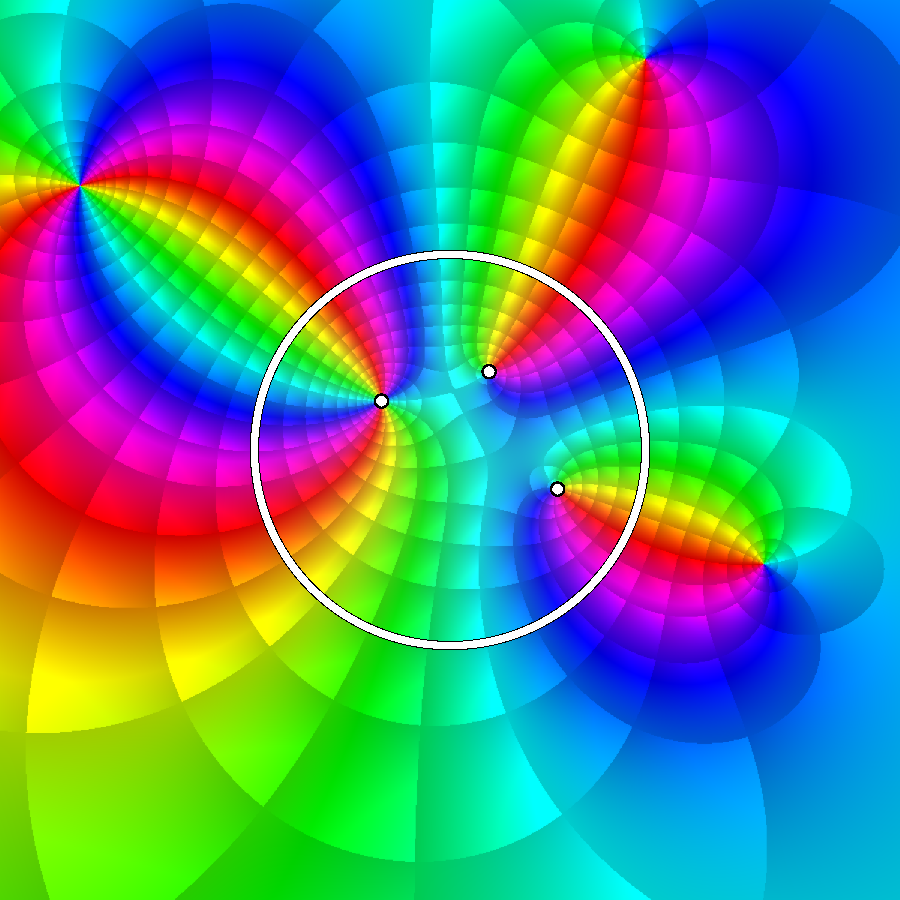
\includegraphics[width=0.3\textwidth]{blaschke_domain_coloring.pdf}
            % \caption{Domain coloring de un producto de Blaschke de grado $3$.}
        \end{figure}
    \end{multicols}



    \note<1>[item]{
        El tercer capítulo de la memoria está dedicado a los productos de Blaschke finitos y a sus propiedades más relevantes.
    }    
    \note<1>[item]{
        Un producto de Blaschke finito es una función de variable compleja con esta forma. Recordando la caracterización de los automorfismos del disco unidad, podemos ver que un producto finito de Blaschke de grado $n$ no es más que un producto de $n$ automorfismos del disco unidad.
    }
    \note<1>[item]{
        Denotaremos con una be caligráfica al conjunto de productos de Blaschke finitos y añadiremos un subíndice para indicar el grado cuando sea necesario.
    }

    \note<2>[item]{
        Como propiedades fundamentales tenemos que 
    }%COMPLETAR: añadir notas
\end{frame}

\subsection{Valencia constante}

\begin{frame}{Valencia constante de los productos de Blaschke finitos}
    $f \in \mathcal{H}\left(\Omega\right)$ es $n$-valente en $\Omega$ si $\forall w \in f(\Omega) :$ la ecuación $f(z) = w$ tiene exactamente $n$ soluciones en $\Omega$ contadas con multiplicidad.

    \vspace{1em}

    \begin{teo}[Valencia constante]
        Si $B \in \mathscr{B}_n$, entonces $B$ es $n$-valente en $\mathbb{D}$.
    \end{teo}

    \vspace{1em}

    \begin{itemize}[itemsep=0.5em]
        \item $B \in \mathscr{B}_n \implies B$ es $n$-valente en $\mathbb{T}$ con soluciones simples.
        \item $B \in \mathscr{B}_n \implies B$ es $n$-valente en $\hat{\C} \setminus \mathbb{D}$.
    \end{itemize}
    %COMPLETAR: añadir notas
\end{frame}

\subsection{Teorema de Fatou}

\begin{frame}{Teorema de Fatou}
    \begin{teo}[Fatou]\label{teo:fatou}
        Si $f \in \mathcal{H}\left(\mathbb{D}\right)$ y $\abs{f(z)} \xrightarrow[\abs{z} \to 1^-]{} 1$, entonces $f \in \mathscr{B}$.
    \end{teo}
    \pause
    \begin{dem}[Idea]
        \begin{minipage}{0.25\textwidth}
            \begin{tikzpicture}[scale=1.8]
                % Unit disk
                \draw (0,0) circle [radius=1];
                % Inner disk K
                \fill[gray!50] (0,0) circle [radius=0.75];
                \draw (0,0) circle [radius=0.75];
                \node at (0.1,0.4) {$\bar{D(0, r)}$};
                % Marked points in K
                \fill (0.15,0.18) circle (0.03);
                \fill (-0.15,0.7) circle (0.03);
                \fill (-0.2,0.1) circle (0.03);
                \fill (-0.6,-0.1) circle (0.03);
                \fill (-0.25,-0.65) circle (0.03);
                \fill (-0.1,-0.22) circle (0.03);
                \fill (0.4,-0.32) circle (0.03);
            \end{tikzpicture}            
        \end{minipage}
        \hfill
        \begin{minipage}{0.7\textwidth}
            \begin{itemize}[wide, itemsep=0.5em]
                \item $\exists r < 1 : \{\text{ceros de }f\} \subset \bar{D(0, r)} \Subset \mathbb{D}$.
                \pause
                \item $\exists \left(z_k\right)_{k=1}^n \subset \mathbb{D} : \{\text{ceros de }f\} = \{z_1, \ldots, z_n\}$.
                \pause
                \item $B \defeq \prod_{k=1}^n \tau_{z_k} \in \mathscr{B}_n$.
                \pause
                \item $\sfrac{f}{B}, \sfrac{B}{f} \in \mathcal{H}\left(\mathbb{D}\right)$ y $\abs{\sfrac{f}{B}}, \abs{\sfrac{B}{f}} \leq 1 \implies \abs{\sfrac{f}{B}} \equiv 1$.
                \pause
                \item $\exists \gamma \in \mathbb{T} : \sfrac{f}{B} \equiv \gamma$, luego $f = \gamma \cdot B \in \mathscr{B}_n$.
            \end{itemize}

            \vspace{-\baselineskip}
            % \vspace{-\belowdisplayskip}
            \hfill\qedsymbol
        \end{minipage}
    \end{dem}

    \note<1>[item]{
        El primer resultado que veremos es este teorema de Fatou, que proporciona una caracterización de los productos de Blaschke finitos como funciones holomorfas en el disco unidad en términos de su comportamiento en la frontera del disco unidad.
    }
    \note<1>[item]{
        Como este teorema se aplica continuamente a lo largo del trabajo y además su demostración es sencilla y representativa de las técnicas que se utilizan en el TFG, he decidido incluir el esquema de la demostración en la presentación. 
    }


    \note<2-3>[item]{
        La segunda condición del teorema implica que la función $f$ no se puede anular cerca de la frontera del disco unidad, por lo que todos sus ceros deben estar contenidos en un disco cerrado.
    }
    \note<3>[item]{
        Como este conjunto es compacto y $f$ es holomorfa no idénticamente nula por la segunda condición, por el principio de los ceros aislados, $f$ solo puede tener un número finito de ceros, digamos $n$ contados con multiplicidad.

        Lo escribo con paréntesis para indicar que los $z_k$ se pueden repetir.
    }
    \note<4-6>[item]{
        Entonces, si definimos $B$ como el producto finito de blaschke dado por esta fórmula, $B$ se anula exactamente en los ceros de $f$ con la misma multiplicidad, luego
    }
    \note<5-6>[item]{
        tanto $\sfrac{f}{B}$ como $\sfrac{B}{f}$ son funciones holomorfas en el disco unidad (por el teorema de la singularidad evitable de Riemann).
    }
    \note<5-6>[item]{
        Además, por el principio del módulo máximo, tenemos estas dos desigualdades que, combinadas, implican que el módulo de $f$ entre $B$ es idénticamente igual a $1$ en el disco unidad.
    }
    \note<6>[item]{
        Como además hecho visto que $f$ entre $B$ es una función holomorfa, al tener módulo constante, debe ser una función constante, es decir, existe un número complejo $\gamma$ de módulo $1$ tal que $f$ es igual a $\gamma$ por $B$, que es un producto de Blaschke finito de grado $n$ y hemos terminado.
    }
\end{frame}

\subsection{Consecuencias del teorema de Fatou y otros resultados relacionados}

\begin{frame}
    \begin{cor}[Caracterización en el álgebra del disco unidad]
        Si $f \in \mathcal{H}\left(\mathbb{D}\right) \cap \mathcal{C}\left(\bar{\mathbb{D}}\right)$ y $f \left(\mathbb{T}\right) \subset \mathbb{T}$, entonces $f \in \mathscr{B}$.
    \end{cor}

    \pause
    \vspace{1em}

    \begin{teo}[Composición de productos de Blaschke finitos]
        Si $B_1 \in \mathscr{B}_{n_1}$ y $B_2 \in \mathscr{B}_{n_2}$, entonces $B_1 \circ B_2 \in \mathscr{B}_{n_1 n_2}$.
    \end{teo}

    \pause
    \vspace{1em}

    \begin{teo}[Caracterización en la clase de Schur]
        Si $f \in \mathscr{S}$ es $n$-valente en $\mathbb{D}$, entonces $f \in \mathscr{B}_n$.
    \end{teo}
    %COMPLETAR: añadir notas
\end{frame}

\section{Aproximación por productos de Blaschke finitos}

\begin{frame}{Aproximación de funciones en la clase de Schur}
    \begin{itemize}
        \item $\mathscr{B}$ es cerrado para la convergencia uniforme en $\mathbb{D}$.
    \end{itemize}

    \pause

    \begin{teo}[Carathéodory]\label{teo:caratheodory}
        $\mathscr{B}$ es denso en $\mathscr{S}$ para la convergencia uniforme sobre compactos de $\mathbb{D}$.
    \end{teo}

    \pause

    \begin{lem}[Auxiliar]
        $f \in \mathscr{S} \implies \forall n \in \N : \exists B_n \in \mathscr{B}_n : \operatorname{ord}(f - B_n, 0) \geq n$. 
    \end{lem}
    %COMPLETAR: añadir notas
\end{frame}


\begin{frame}
    
\end{frame}


\begin{frame}
    
\end{frame}

% =========================
\begin{frame}[standout]
    \Huge
    Gracias

    \vspace{0.3cm}

    \normalsize
    Preguntas
\end{frame}

\end{document}